\setchapterpreamble[u]{\margintoc}
\chapter{固件烧录与配置}
\labch{flandco}

\setlength\parindent{2em} 上一章中,适用于本项目的操作系统与应用程式的编译与准备已经完成,本章将介绍将操作系统与应用程式的二进制文件烧录到单片机上的过程,并将其配置到合适状态的过程。本章最后会将整个开关电路组装并且进行试验,为下一章的电路部署做准备。

\section{固件的准备与烧录}

\setlength\parindent{2em} 上一章中已经将所需的操作系统与应用程式进行选择与编译,最终得到三个二进制文件。下一步,将三个二进制文件合成一个,暂且称之为一个完整的“固件”——即写入可擦写可编程只读存储器中的程序。它的一部分十六进制编码大致如下:\reffig{normalhex}

\begin{figure*}[h!]
	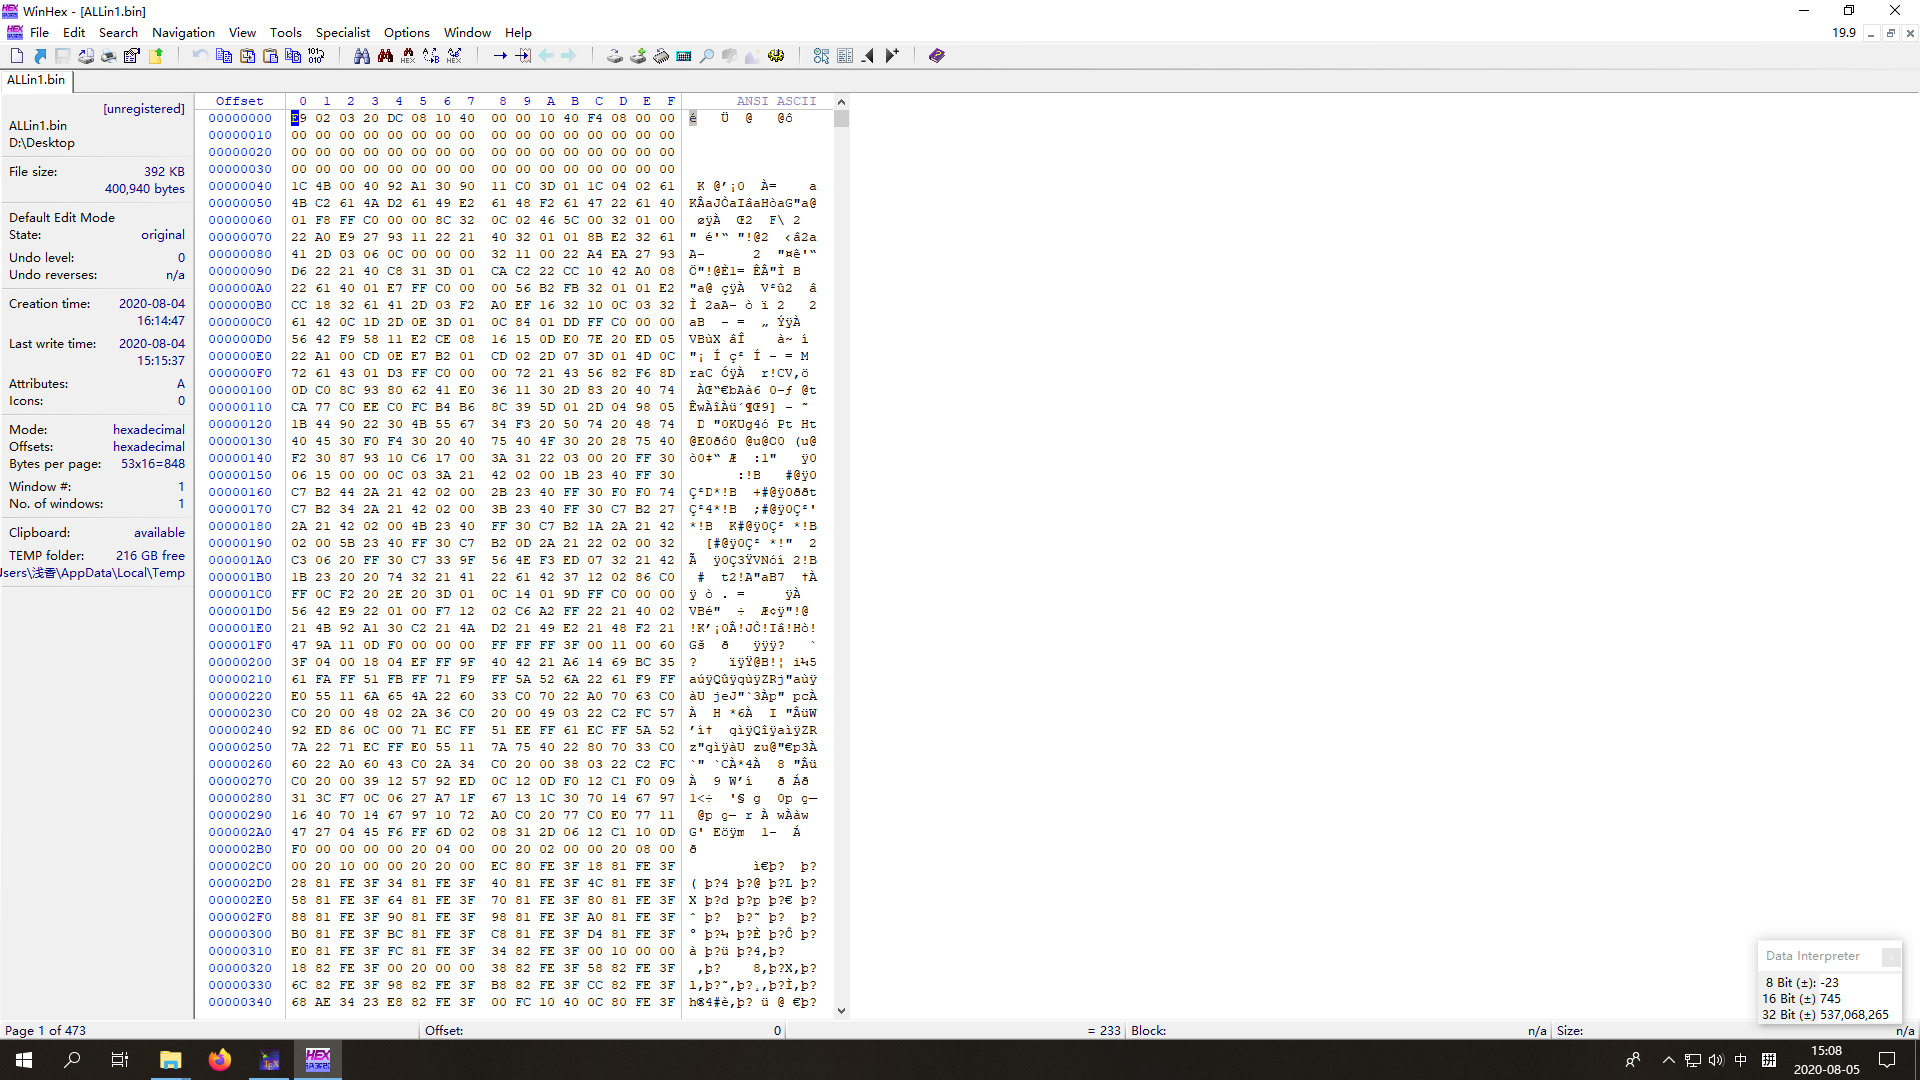
\includegraphics[width=\textwidth]{hex}
	\caption[hex]{固件的十六进制编码的一部分}
	\labfig{normalhex}
\end{figure*}

\par 固件已经准备完成,下一步就是把它烧录的微控单元中,即将其写入微控单元的储存器。根据Espressif Inc.官方提供的文档,可以下载到适用于ESP芯片的烧录程序\sidenote{\url{https://www.espressif.com/sites/default/files/tools/flash_download_tool_v3.8.5.zip}}。将其下载后,准备UART转换至USB的转换器,以通过通用异步收发传输器\sidenote{通用异步收发传输器(Universal Asynchronous Receiver/Transmitter),通常称作UART,是一种通用串行数据总线,用于异步通信。该总线双向通信,可以实现全双工传输和接收。它将要传输的资料在串行通信与并行通信之间加以转换。作为把并行输入信号转成串行输出信号的芯片,UART通常被集成于其他通讯接口的连结上。}与计算机之间进行串行通信。本次使用的转换器芯片为CP2104,为CP210x类芯片之一,比较常用的串行通信芯片。将其与计算机连接后,运行烧录程序,预先在端口设置中将调制速率调节至115200。在烧录程序中清除微控单元的闪存芯片,填充为0,再将准备好的固件从0x0,即第零扇区开始烧写,整个过程需要几分钟,如图\reffig{normalflash}所示:

\begin{figure*}[h!]
	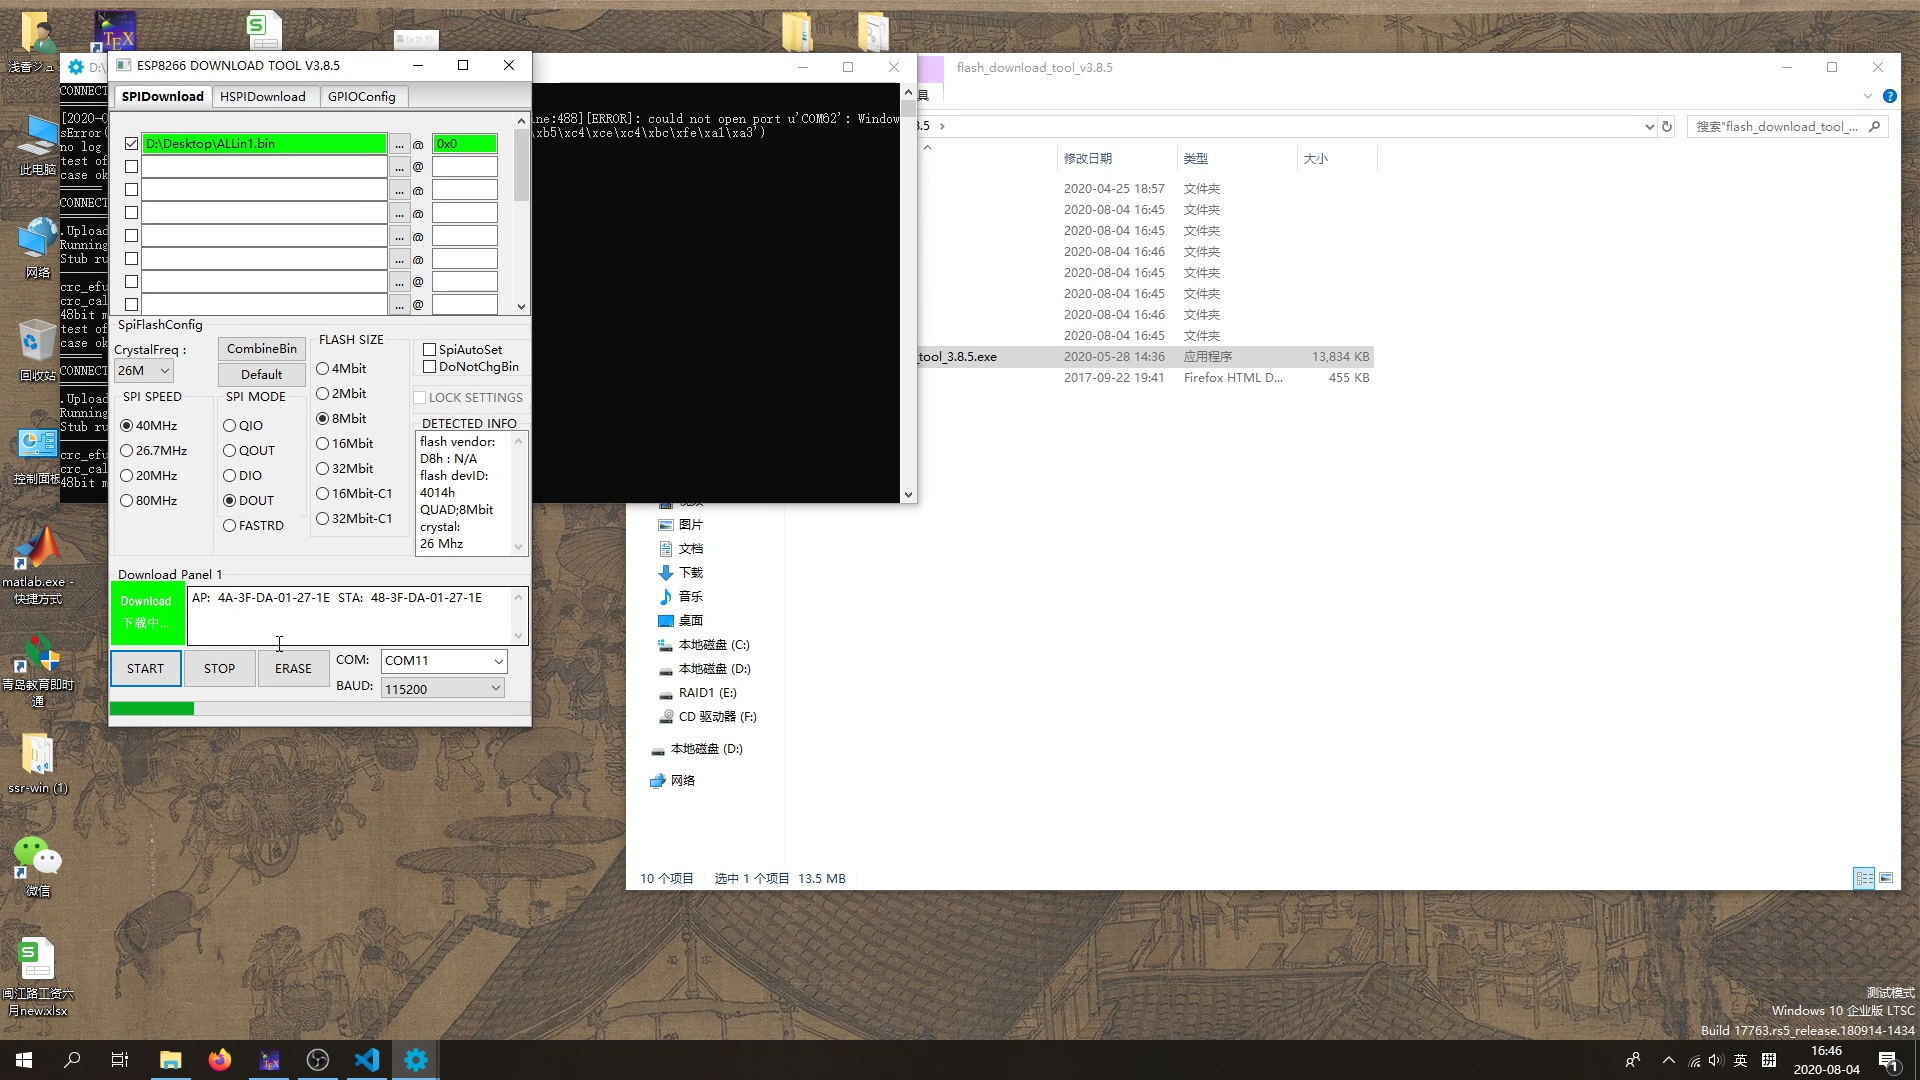
\includegraphics[width=\textwidth]{flash}
	\caption[flash]{固件烧写的过程}
	\labfig{normalflash}
\end{figure*}


\begin{marginfigure}[0cm]
	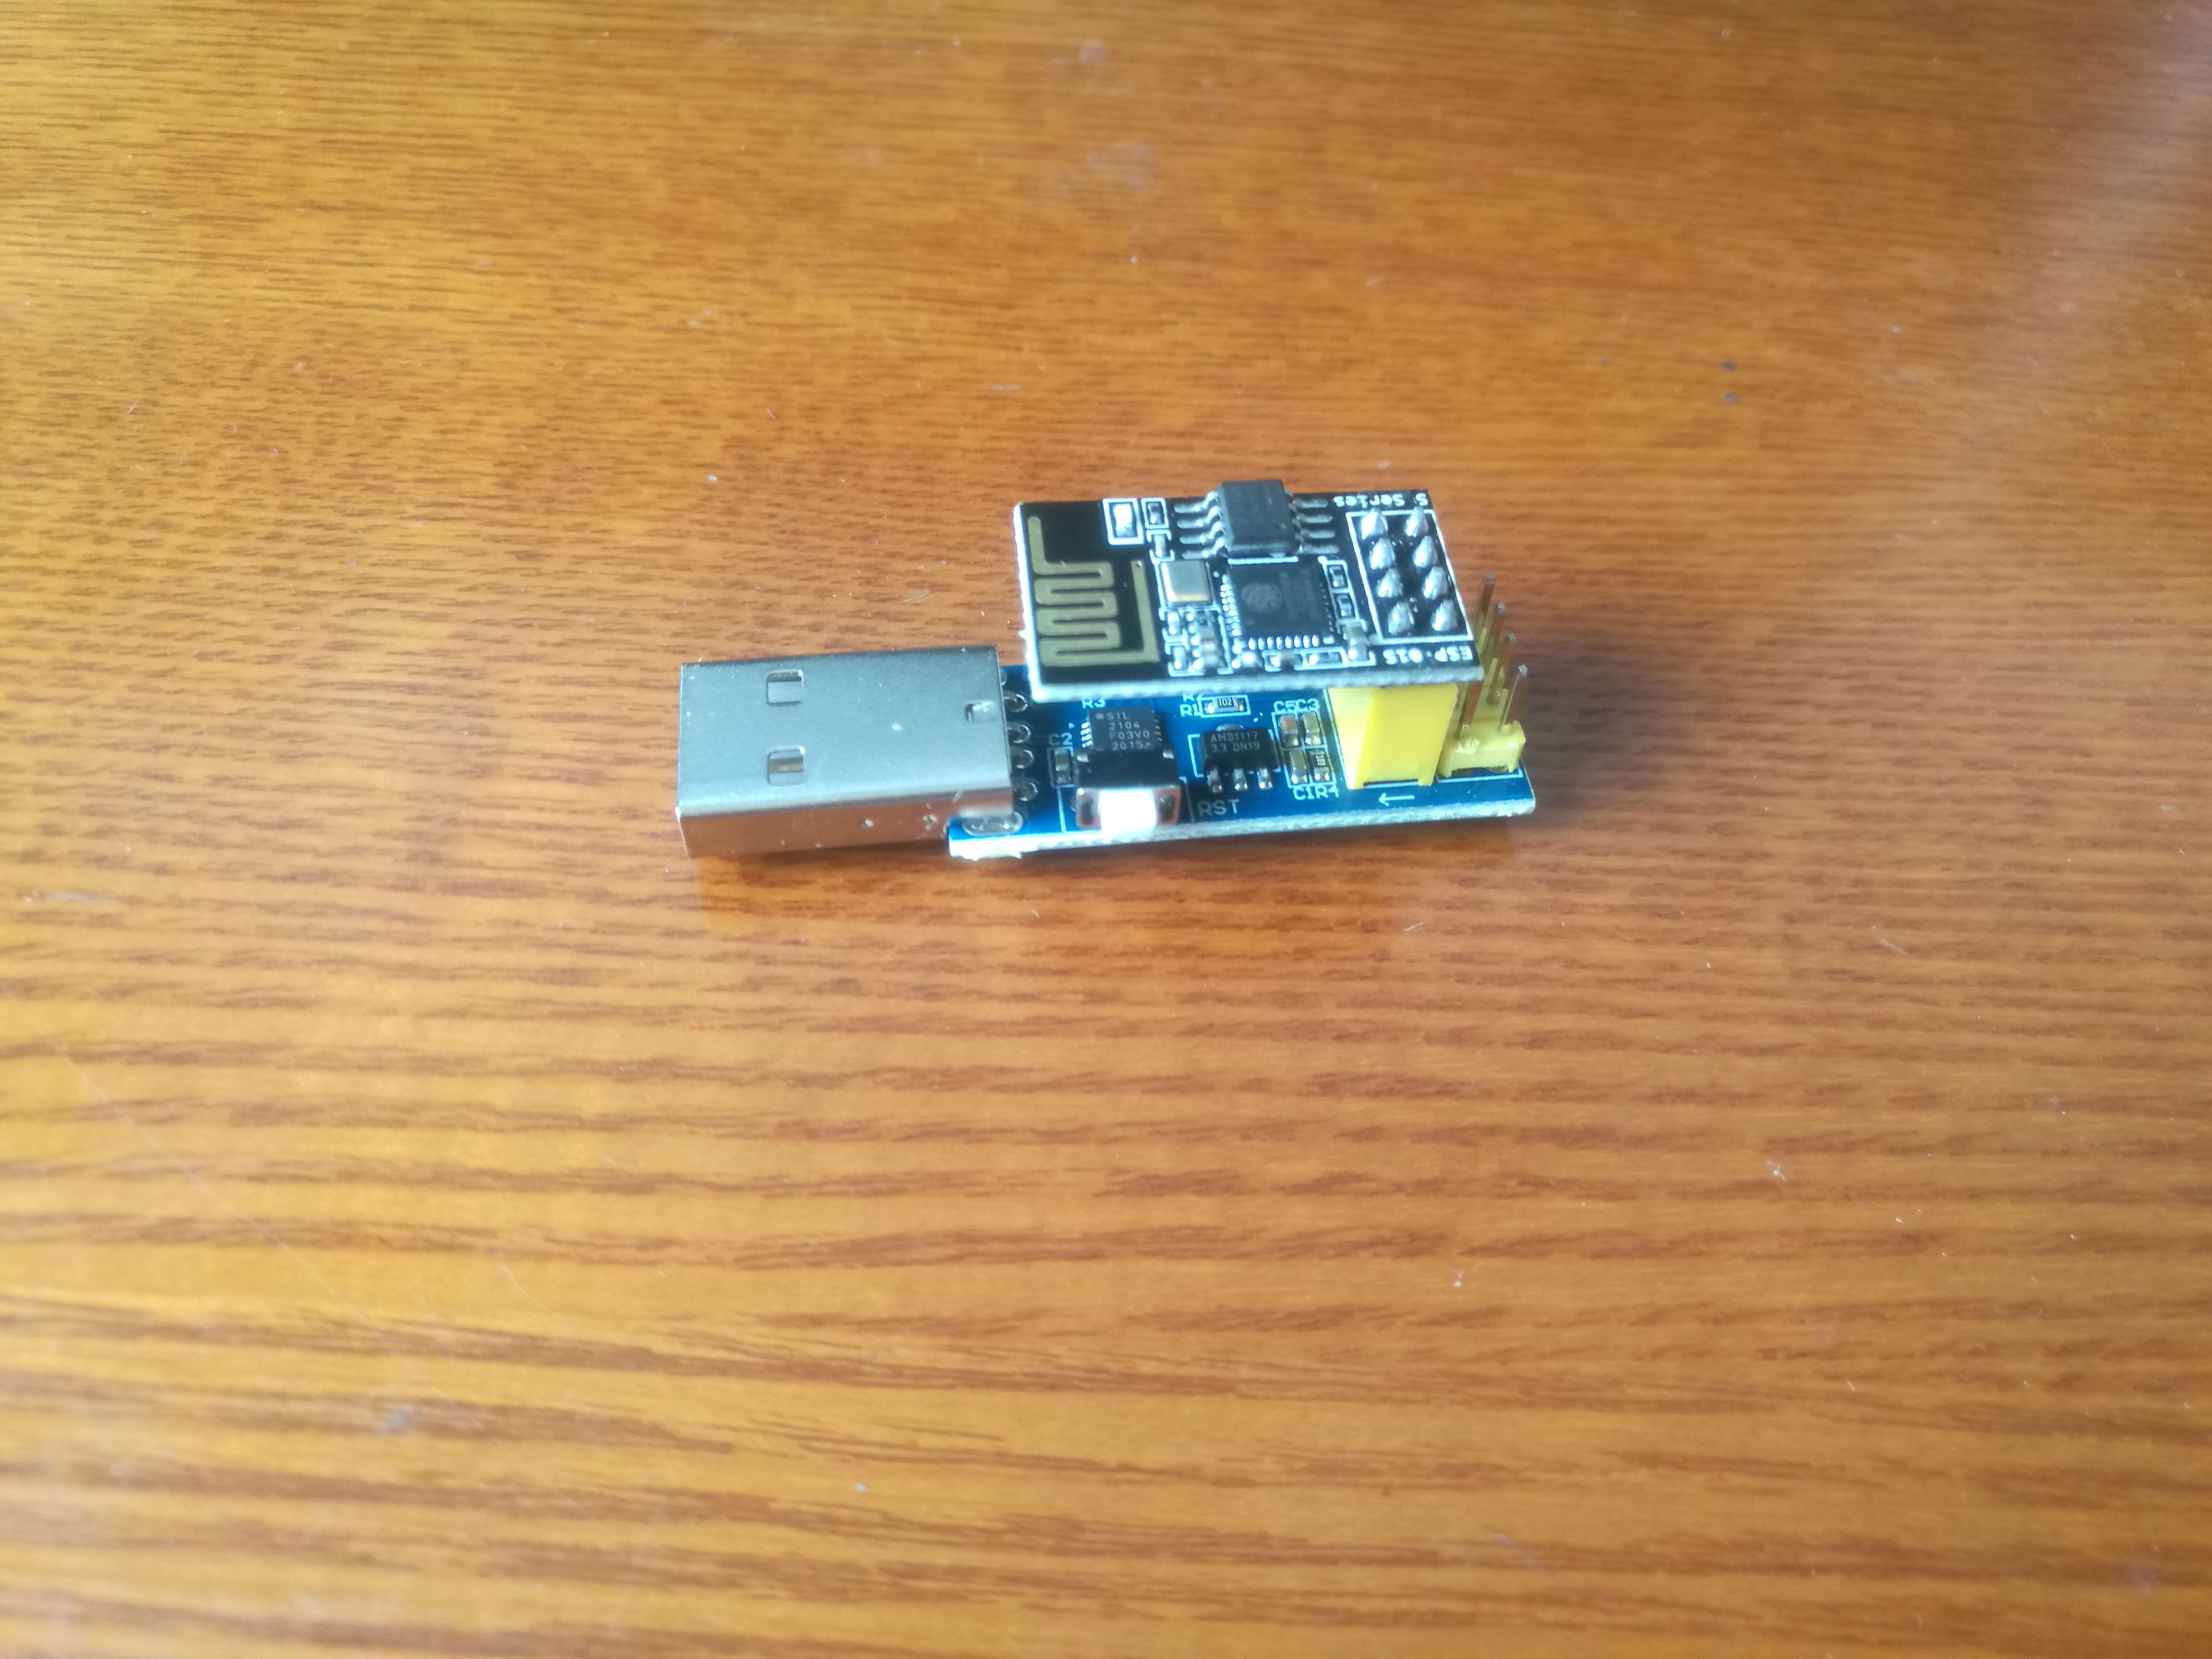
\includegraphics{flasher}
	\caption[flasher]{微控单元与烧写器}
\end{marginfigure}

\par 至此,烧录完成。将微控单元与烧写器断开,将其接至继电器模块上的端口。并且将继电器模块上的供电用端子座连接上5V直流电源,此时继电器应该突然闭合又断开,可以在附近搜索到SSID为HAA开头的Wi-Fi协议无线网络信号,表示烧录成功。

\section{应用程式的配置}

\setlength\parindent{2em} 烧录成功后,进入配置阶段。根据HAA官方位于GitHub上的Wiki,需要编写json来对设备进行配置,或者说是编程;将连接的设备、电平的高低、触发器、指示灯等等进行控制。在硬件电路的设计中,按照最后的设计图,继电器闭合对应着GPIO0的低电平,若GPIO0为高电平,则继电器断开,或者说是公共端与常闭端导通。于是得到如下配置:继电器与GPIO0连接;继电器正常状态为GPIO0的高电平;继电器在电路通电时默认断开。其它按照Wiki中的设置,未作修改。最终完整的json文件如下图\reffig{normaljson}所示:

\begin{figure*}[h!]
	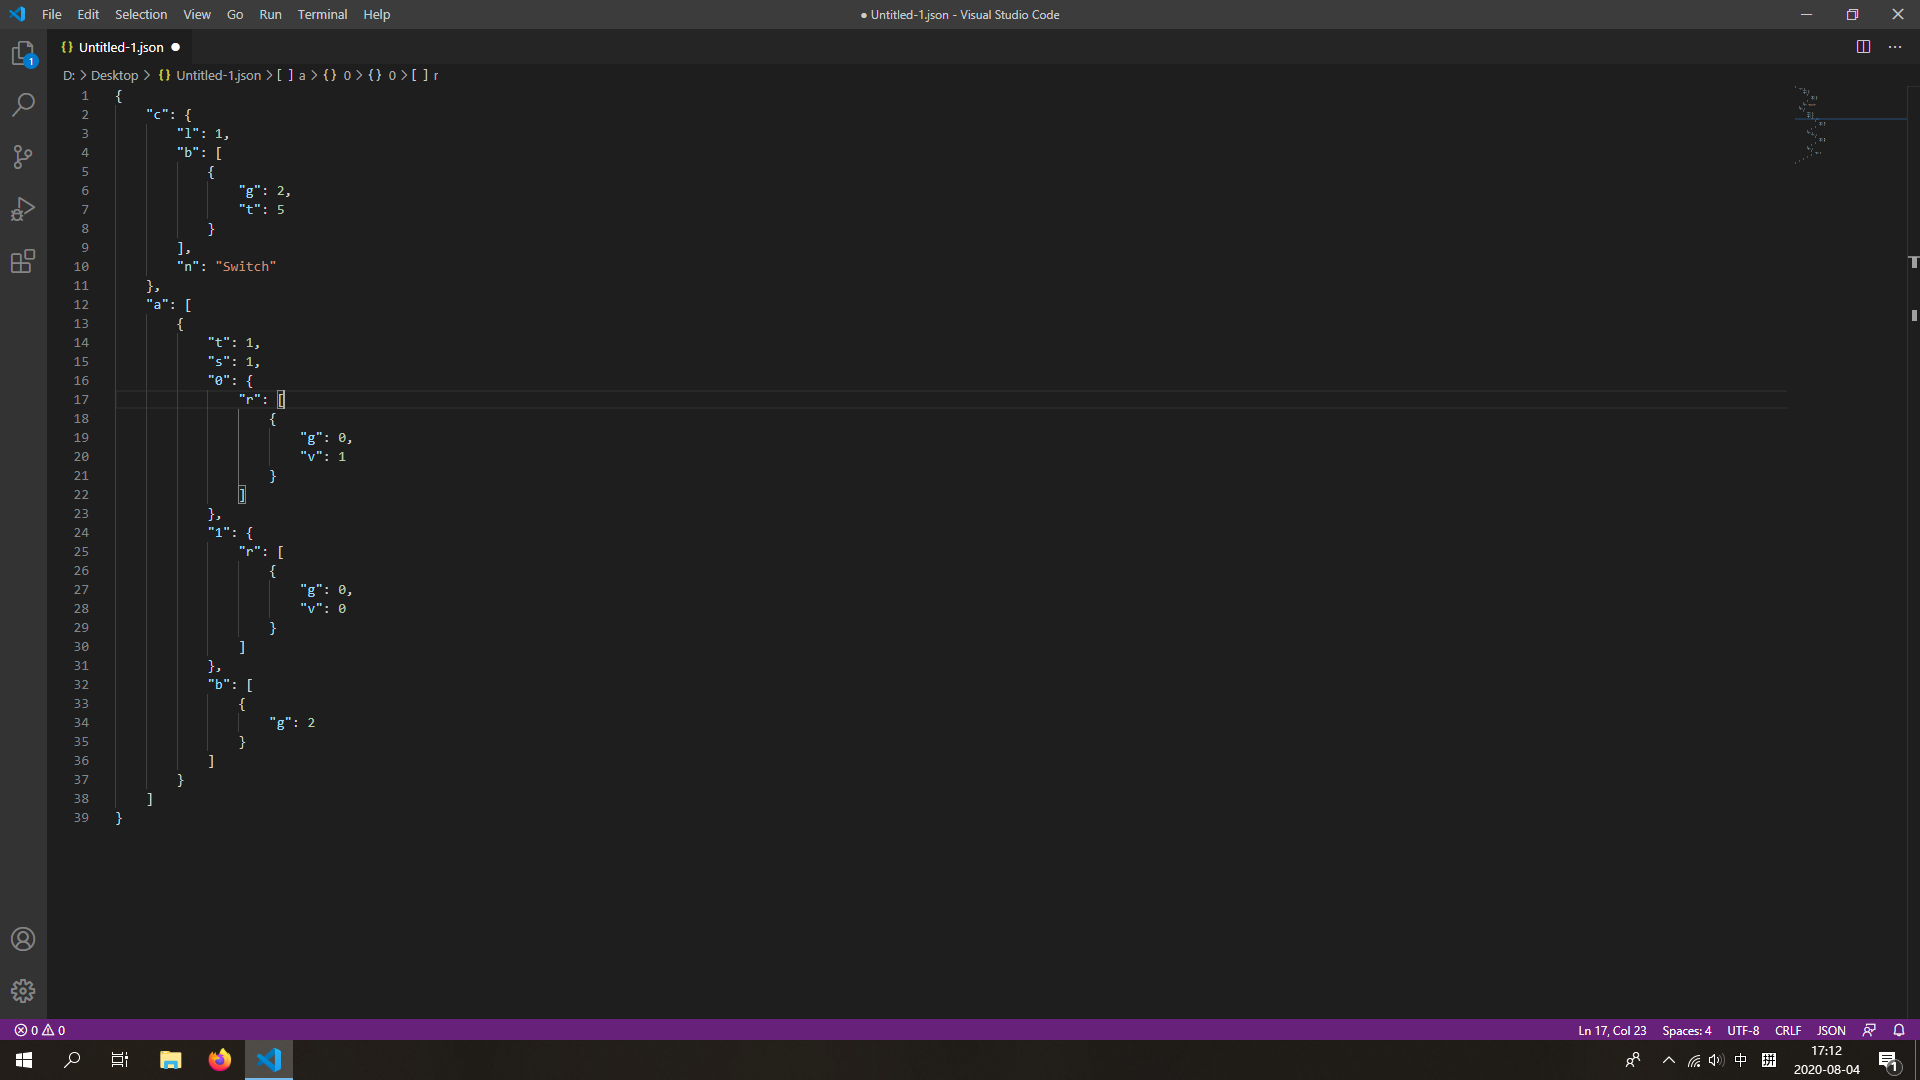
\includegraphics[width=\textwidth]{json}
	\caption[json]{完整的json配置文件}
	\labfig{normaljson}
\end{figure*}

\par 接下来进行设备的配置。将微控单元与继电器模块连接后,模块上的端子座通上5V直流电,此时可以在附近搜索到没有加密的Wi-Fi协议无线网络。加入无线网路,用浏览器访问http://192.168.4.1/,这个网址可以在HAA的Wiki上找到,以为本设备,为这个应用程式的配置页面。进入后如图\reffig{normalconf}所示:

\begin{figure*}[h!]
	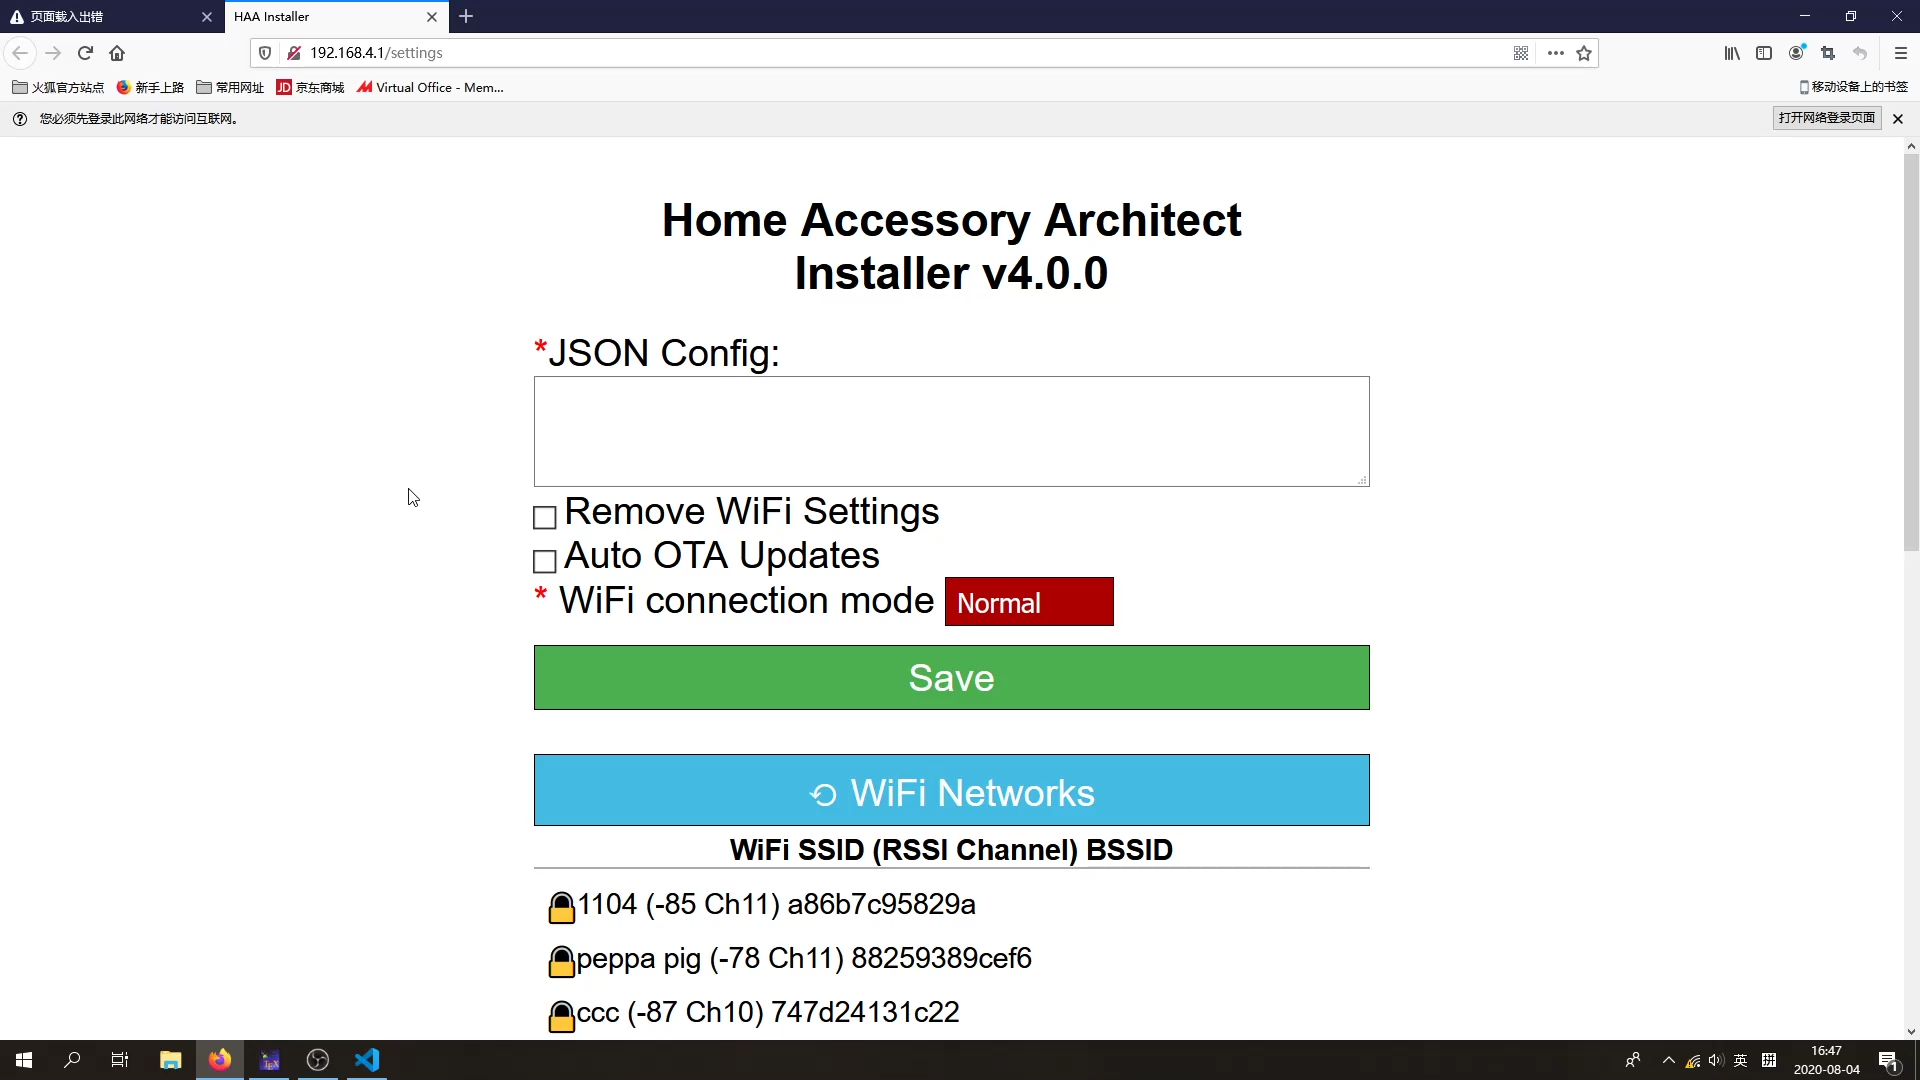
\includegraphics[width=\textwidth]{conf}
	\caption[conf]{微控单元应用程式的配置页面}
	\labfig{normalconf}
\end{figure*}

\par 接下来就很简单,将json配置填写到顶部JSON Config一栏,最好将json格式化为一行,这样可以节省对储存器的占用——根据官方Wiki所说。在下面选择所要连接的无线网络(仅支持Wi-Fi协议),输入密码,点击Save,配置就完成了。

\par 然后就需要等待了。由于微控单元的处理能力极为低下,所以其将配置应用到设备并接入无线网络所用的时间相对较长,大概需要十多分钟才可以进行下一步的连接。当其配置完成后,微控单元上的LED指示灯应该会闪烁一下。

\begin{marginfigure}[0cm]
	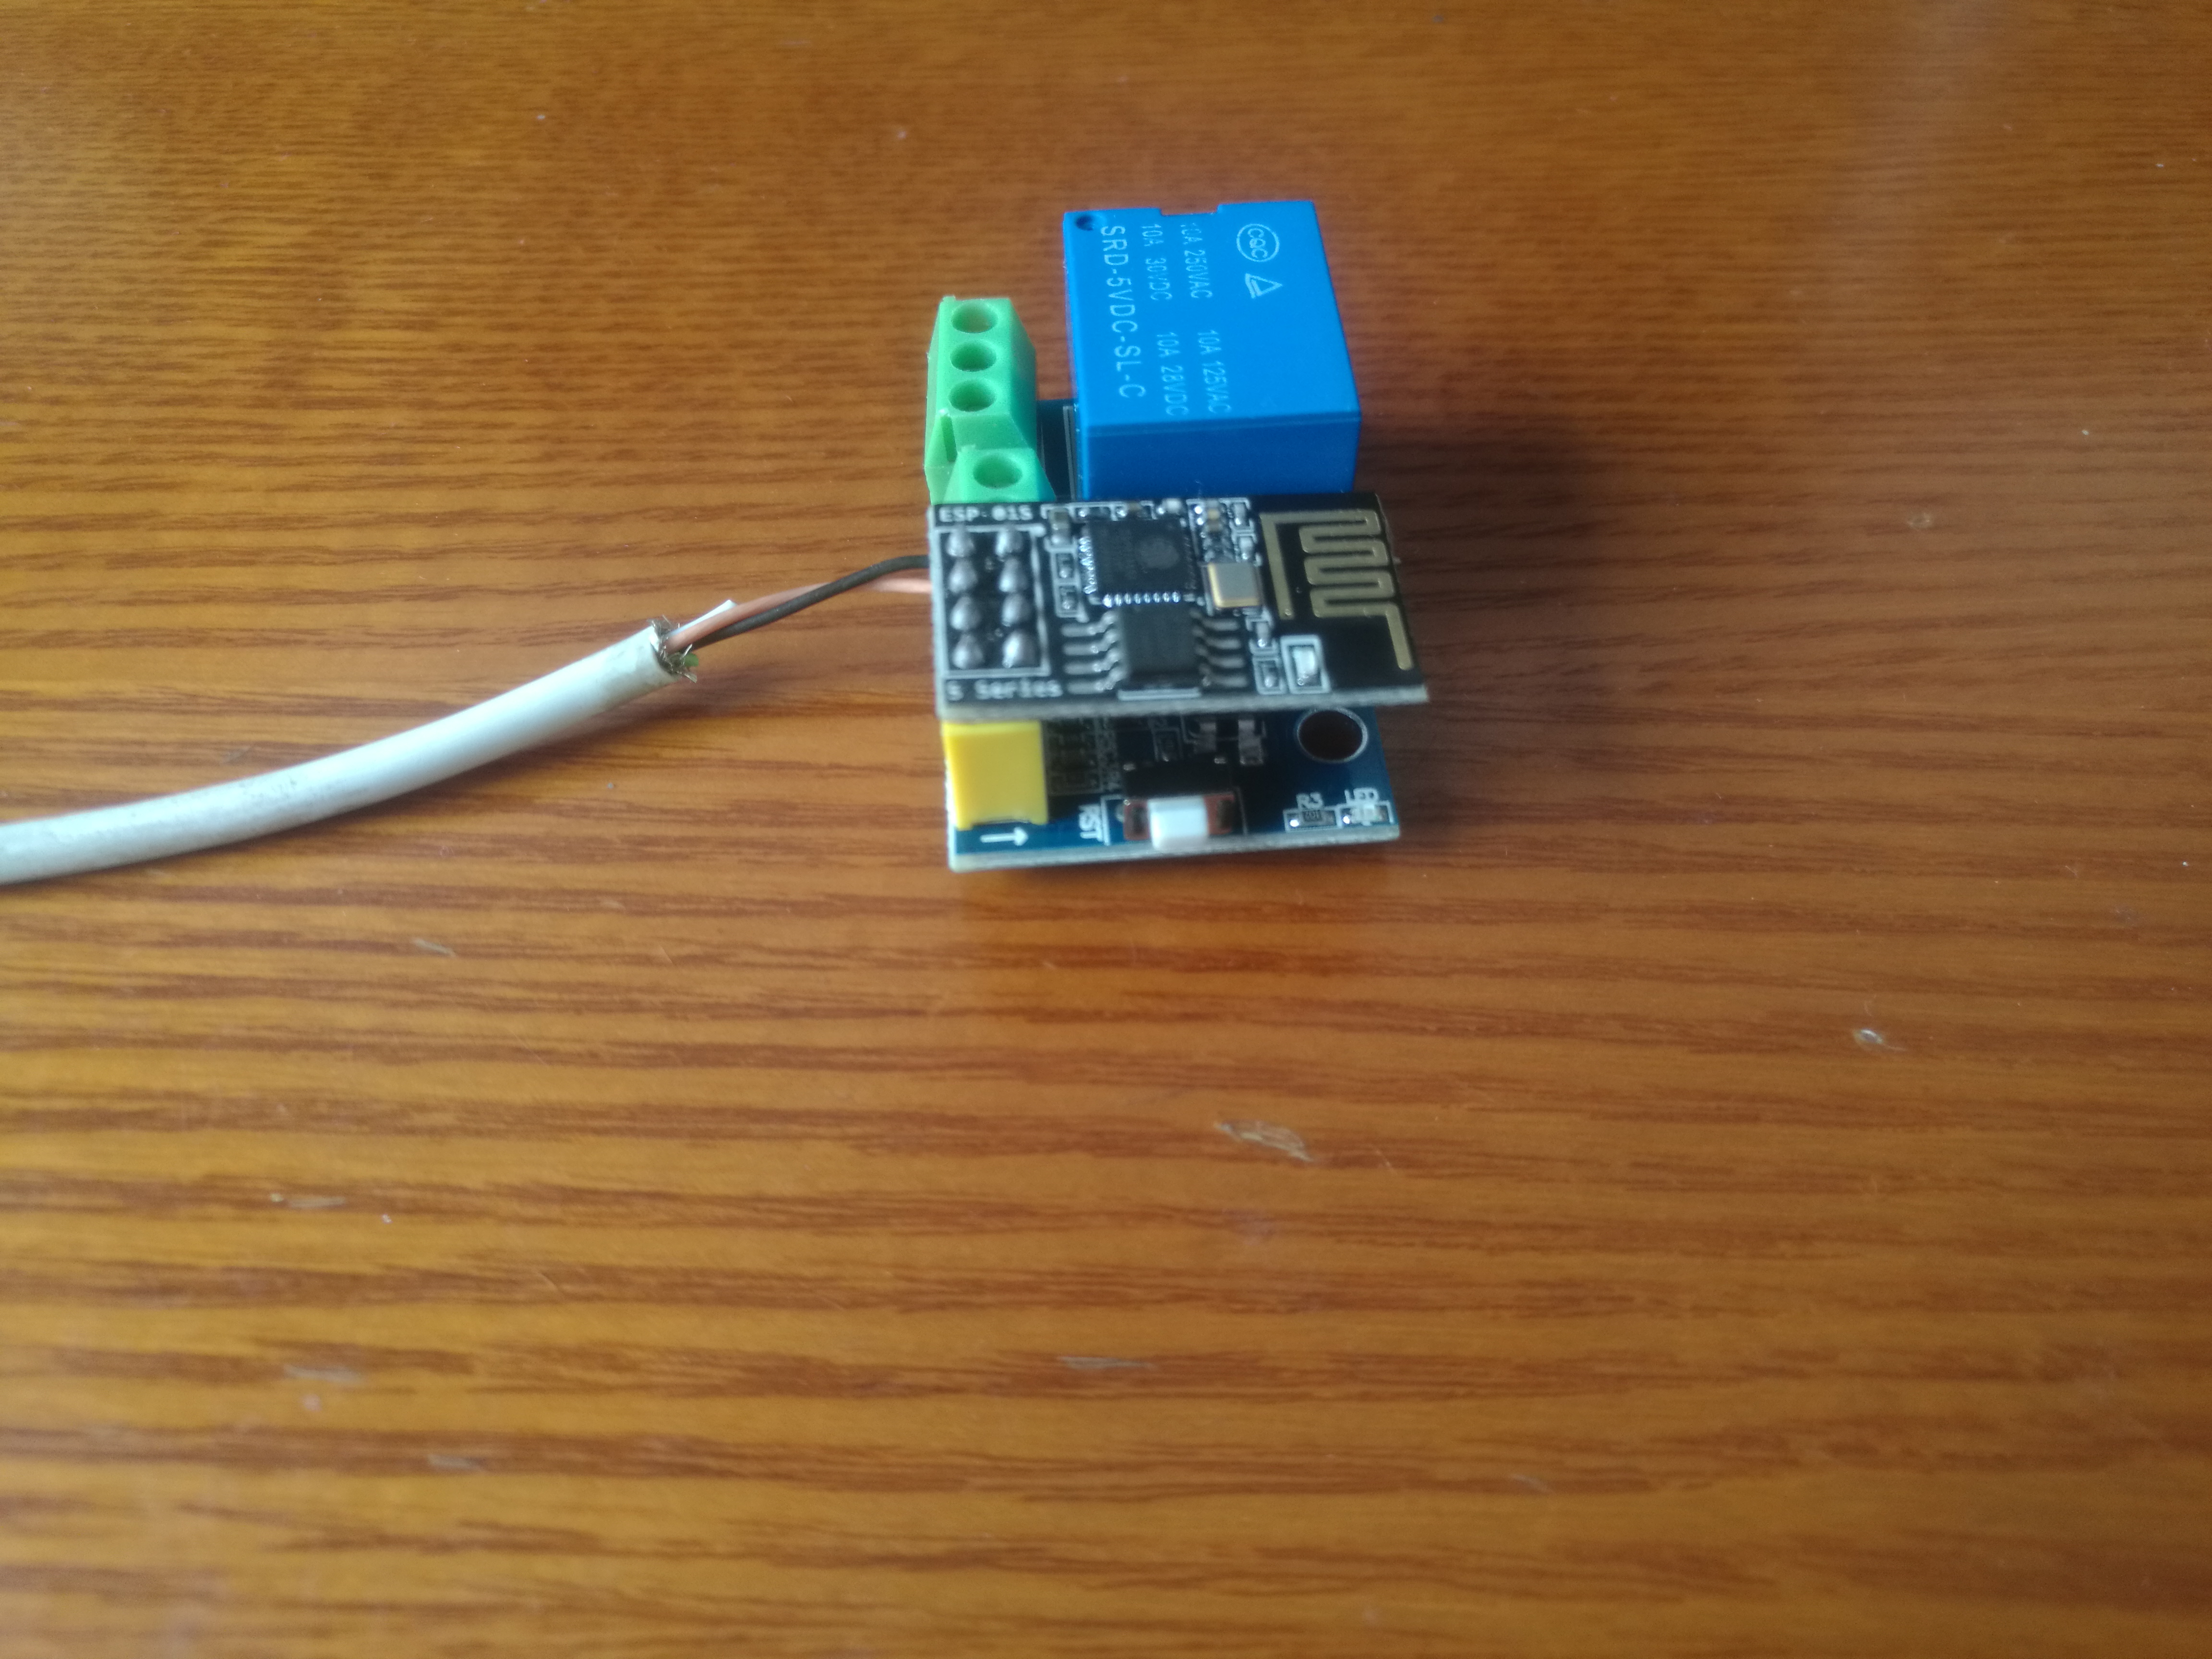
\includegraphics{all}
	\caption[all]{微控单元与继电器}
\end{marginfigure}

\section{继电器电路与客户端的连接}

\setlength\parindent{2em} 应用程式配置好后等待其自动应用配置,然后即可与Apple HoneKit客户端进行连接。按照Apple Inc.官方开发文档,对开发与调试描述地很详细,在此要做的就是将微控单元与Apple智能设备连接到同一无线网络下,上一节已经将微控单元接入网络。此时,打开Apple智能设备中的“Home”应用程序,非特殊情况,仅支持运行iOS8及以上的Apple设备。点击“Add Accessory”。由于没有提供可供扫描的QR二维码,选择“Don't Have a Code”,此时一个名为HAA开头的设备应该出现在屏幕上。根据HAA官方Wiki,所有的HAA应用程式所用的连接代码是一样的。如图\reffig{normalcode}所示。

\begin{marginfigure}[0cm]
	
\includegraphics{code}
	\caption[code]{连接代码}
	\labfig{normalcode}
\end{marginfigure}

\par 输入代码后,会自动连接,大概需要一分多钟。连接后,如图\reffig{normalresult}所示,即可自由控制该继电器,继电器模块上的LED表示继电器的状态,若灯亮则表示继电器导通(公共端与常闭端导通);反之,则公共端与常开端导通。若测试有效,则表明电路正常工作,可以进行下一步的电路部署工作了。

\begin{figure*}[h!]
	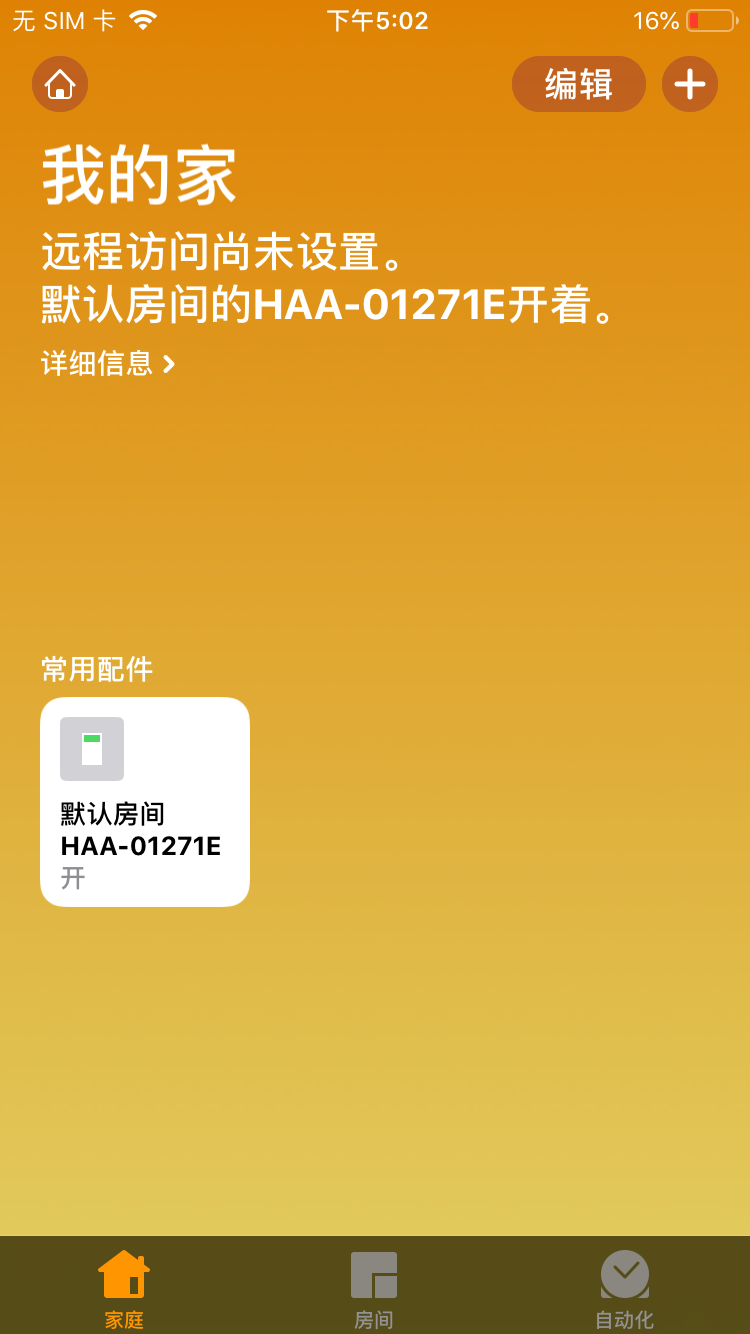
\includegraphics[width=\textwidth]{result}
	\caption[result]{连接成功}
	\labfig{normalresult}
\end{figure*}
